\uuid{Xqjl}
\exo7id{7286}
\titre{exo7 7286}
\auteur{mourougane}
\organisation{exo7}
\datecreate{2021-08-10}
\isIndication{false}
\isCorrection{false}
\chapitre{Géométrie affine euclidienne}
\sousChapitre{Géométrie affine euclidienne du plan}
\module{Géométrie}
\niveau{L2}
\difficulte{}

\contenu{
\texte{
On considère un cercle \(\mathcal{C}\) de centre \(O\) et deux points 
distincts \(A\) et \(B\). On veut construire au compas seul les points 
d'intersection du cercle \(\mathcal{C}\) et de la droite \((AB)\).
}
\begin{enumerate}
    \item \question{Si \(O \notin (AB)\), expliquer comment construire ces deux points. 
(\emph{Indication :} on pourra construire le symétrique du cercle \(\mathcal{C}\) 
par rapport à la droite \((AB)\), en utilisant 
l'exercice~\ref{sym-compas-seul}.)}
    \item \question{Si \(O \in (AB)\), on se ramène à une intersection de cercles en 
utilisant une inversion. Plus précisément, on considère la construction 
suivante.

\begin{center}
    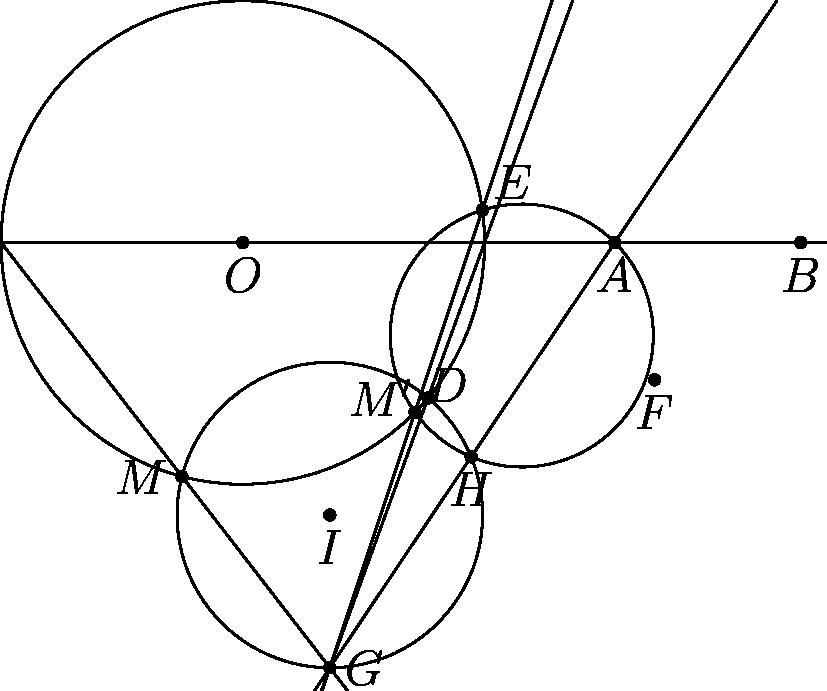
\includegraphics[scale=1]{images/Xqjl-1}
\end{center}

% [[figure asymptote]]

%\begin{center}
%\begin{asy}
%size(7cm, 0);
%point O = (0, 0); dot("\(O\)", O, S);
%point A = (2, 0); dot("\(A\)", A, S);
%point B = (3, 0); dot("\(B\)", B, S);
%circle C0 = circle(O, 1.3); draw(C0);
%draw(line(A, B));
%point O1 = (1.5, -0.5);
%circle C1 = circle(O1, abs(A - O1)); draw(C1);
%point[] DE = intersectionpoints(C0, C1);
%dot("\(D\)", DE[0], NE); dot("\(E\)", DE[1], NE);
%line L0 = line(DE[0], DE[1]); draw(L0);
%point F = reflect(L0) * O; dot("\(F\)", F, S);
%point G = rotate(60, F) * O; dot("\(G\)", G, E);
%line L1 = line(A, G); draw(L1);
%point[] AH = intersectionpoints(C1, L1);
%point H = (AH[0] == A) ? AH[1] : AH[0]; dot("\(H\)", H, S);
%point I = intersectionpoint(bisector(segment(G, H)),
%      perpendicular(G, line(O, A)));
%dot("\(I\)", I, S);
%circle C2 = circle(I, abs(G - I)); draw(C2);
%point[] M = intersectionpoints(C0, C2);
%dot("\(M\)", M[0], W); dot("\(M'\)", M[1], W);
%draw(line(G, M[0])); draw(line(G, M[1]));
%\end{asy}
%\end{center}

Soit \(\mathcal{C}'\) un cercle passant par \(A\), qui coupe \(\mathcal{C}\) 
en deux points \(D\) et \(E\). Soit \(F\) le symétrique de \(O\) par rapport 
à la droite \((DE)\), et soit \(G\) un point tel que le triangle \(OFG\) soit 
équilatéral. Montrer que \(G \in (DE)\) et expliquer comment le construire au 
compas seul.}
    \item \question{Montrer que \(G\) a la même puissance par rapport à \(\mathcal{C}\) 
et à \(\mathcal{C}'\). En déduire qu'il existe une inversion \( \iota\) de 
centre \(G\) telle que \( \iota(\mathcal{C}) = \mathcal{C}\) et 
\( \iota(\mathcal{C}') = \mathcal{C}'\).}
    \item \question{On note \(\mathcal{C}''\) l'image de la droite \((OA)\) par 
l'inversion \( \iota\) (en ajoutant son centre \(G\) pour avoir un cercle), 
et on note \(I\) le centre de \(\mathcal{C}''\). Montrer que les droites 
\((GI)\) et \((OA)\) sont orthogonales.}
    \item \question{Soit \(H\) l'intersection du cercle \(\mathcal{C}'\) et de la 
droite \((AG)\) qui n'est pas \(A\). Montrer que \( \iota(A) = H\).}
    \item \question{Montrer que \(I\)~est sur la médiatrice du segment \([GH]\). Comment 
construire au compas seul deux points de cette médiatrice?}
    \item \question{Comment construire deux points de la perpendiculaire à \((OA)\) 
passant par \(G\)? (\emph{Indication :} construire le symétrique de \(G\) par rapport 
à \((OA)\).)}
    \item \question{Montrer que \(I\) est l'intersection de la médiatrice de \([GH]\) et 
de la perpendiculaire à \((OA)\) passant par \(G\) (voir 
l'exercice~\ref{inter-droites-compas-seul} pour comment construire cette 
intersection au compas seul).}
    \item \question{En déduire comment construire \(\mathcal{C}''\). (\emph{Indication :} 
\(G \in \mathcal{C}''\).)}
    \item \question{On note \(M\) et \(M'\) les points d'intersection de \(\mathcal{C}\) 
et \(\mathcal{C}'\). Montrer que \( \iota(M)\) et \( \iota(M')\) sont les points 
d'intersection de \(\mathcal{C}\) et \((AB)\).}
    \item \question{Montrer que \( \iota(M)\) est l'intersection de \(\mathcal{C}\) et de 
la droite \((GM)\), autre que \(M\).}
\end{enumerate}
}
